\documentclass[11pt,a4paper]{article}
\usepackage[margin=20mm,headheight=15pt]{geometry}
\usepackage{fontspec,graphicx,xcolor,fancyhdr,listings,hyperref,array}
\setmainfont{Liberation Sans}
\setmonofont{Liberation Mono}
\definecolor{navy}{HTML}{103253}
\definecolor{blue}{HTML}{0068AF}
\definecolor{pale}{HTML}{F4F7FA}
\hypersetup{colorlinks=true,linkcolor=blue,urlcolor=blue,pdftitle={MXB362 PST2 Portfolio - Owen Ferguson},pdfauthor={Owen Ferguson}}
\pagestyle{fancy}\fancyhf{}\renewcommand{\headrulewidth}{0pt}
\renewcommand{\footrulewidth}{0.3pt}
\fancyfoot[L]{\scriptsize\color{navy} MXB362 PST2 Portfolio | Owen Ferguson | n11595744}
\fancyfoot[R]{\scriptsize Page \thepage}
\setlength{\parindent}{0pt}\setlength{\parskip}{7pt}
\lstset{basicstyle=\ttfamily\fontsize{8}{10}\selectfont,breaklines=true,breakatwhitespace=false,columns=fullflexible,keepspaces=true,showstringspaces=false,backgroundcolor=\color{pale},frame=single,rulecolor=\color{pale},numbers=left,numberstyle=\tiny\color{gray},numbersep=6pt,xleftmargin=5mm,framesep=3mm,tabsize=2}
\newcommand{\task}[2]{\clearpage{\LARGE\bfseries\color{navy} #1}\par #2\par}
\newcommand{\figpage}[3]{\clearpage{\Large\bfseries\color{navy} #1}\par\vspace{5mm}\begin{center}\includegraphics[width=\linewidth,height=0.75\textheight,keepaspectratio]{#2}\end{center}{\small #3}\par}
\newcommand{\needspace}[1]{}
\begin{document}
\begin{center}\vspace*{3mm}{\large\color{blue} MXB362}\par\vspace{8mm}
{\Huge\bfseries\color{navy} Computer Lab Portfolio}\par
{\Large\color{blue} Problem Solving Task 2 -- Weeks 8 to 11}\par\vspace{10mm}
\begin{tabular}{|p{42mm}|p{105mm}|}\hline
\textbf{Student}&Owen Ferguson\\[3mm]\hline
\textbf{Student number}&n11595744\\[3mm]\hline\end{tabular}
\end{center}\vspace{6mm}
{\LARGE\bfseries\color{navy} Portfolio contents}\par
{\large\bfseries\color{blue} Week 8 -- Volume Visualisation 2}\par
Task 1: Greyscale stag beetle volume rendering (R)\\
Task 2: Coloured stag beetle isosurface (MATLAB)\\
Additional output: Rotating isosurface animation\par
{\large\bfseries\color{blue} Week 9 -- Visualising Uncertainty}\par
Task 1: Larval dispersal uncertainty animation (MATLAB)\\
Task 2: Three forms of fishery uncertainty (R)\par
{\large\bfseries\color{blue} Week 10 -- Vector Visualisation}\par
Task 1: Direct vector field (quiver plot)\\
Task 2: Poor and improved streamlines\\
Task 3: Line integral convolution, including optional extensions\par
{\large\bfseries\color{blue} Week 11 -- Visualising High Dimensional Data}\par
Task 1: Iris scatter plot matrix\\
Task 2: Principal component projection\\
Task 3: LDA projection vector and Fisher criterion\\
Task 4: Visualising species separation
\task{Week 8 -- Volume Visualisation 2}{Task 1: Produce a greyscale visualisation of the internal and external structure of the stag beetle, viewed from below.}
\needspace{35mm}{\large\bfseries\color{blue} Task 1 -- R volume renderer}\par{\small Source: \texttt{submission/code/week8\_volume.R (run from week8)}}\par
\lstinputlisting{code/week8_volume.R}
The renderer sums voxel intensities along the third dimension, implementing additive blending along parallel viewing rays. The resulting greyscale projection shows overlapping internal and external structures. The matrix is rotated before display.
\figpage{Task 1 -- Greyscale volume projection}{figures/beetle_greyscale.png}{Saved R output: greyscale additive projection of the stag beetle.}
\task{Week 8 -- Coloured isosurface}{Task 2: Render a coloured isosurface with a suitable threshold and viewing angle.}
\needspace{35mm}{\large\bfseries\color{blue} Task 2 -- MATLAB isosurface}\par{\small Source: \texttt{week8/practical8.m}}\par
\lstinputlisting{../week8/practical8.m}
The selected isovalue is 400; the volume is subsampled every third voxel and reversed along the third axis.
\figpage{Task 2 -- Stag beetle isosurface}{../week8/prac8Stag.png}{Saved MATLAB output with a red surface and Gouraud lighting; an oblique view reveals the head, mandibles, legs and body.}
\task{Week 8 -- Additional animation}{Animation file: \texttt{week8/stag\_beetle\_rotation.mp4}.}
\needspace{35mm}{\large\bfseries\color{blue} Rotating isosurface -- MATLAB}\par{\small Source: \texttt{week8/practical8vid.m}}\par
\lstinputlisting{../week8/practical8vid.m}
The animation rotates the isosurface through 720 views at 40 frames per second with a headlight that follows the camera. The still image on the preceding page represents the same isosurface task.
\task{Week 9 -- Visualising Uncertainty}{Task 1: Animate the uncertainty surrounding a larval cloud over time.}
\needspace{35mm}{\large\bfseries\color{blue} Task 1 -- MATLAB larval animation}\par{\small Source: \texttt{week9/P9Task1.m}}\par
Animation file: \texttt{week9/LarvalDispersal.gif}. The following page shows four representative frames; the full temporal output is in the GIF.
\begingroup\lstset{basicstyle=\ttfamily\fontsize{7.5}{9}\selectfont}\lstinputlisting{../week9/P9Task1.m}\endgroup
Green points show individual larval positions and the red convex hull outlines their spatial extent.

\clearpage{\Large\bfseries\color{navy} Task 1 -- Larval dispersal animation}\par\begin{center}
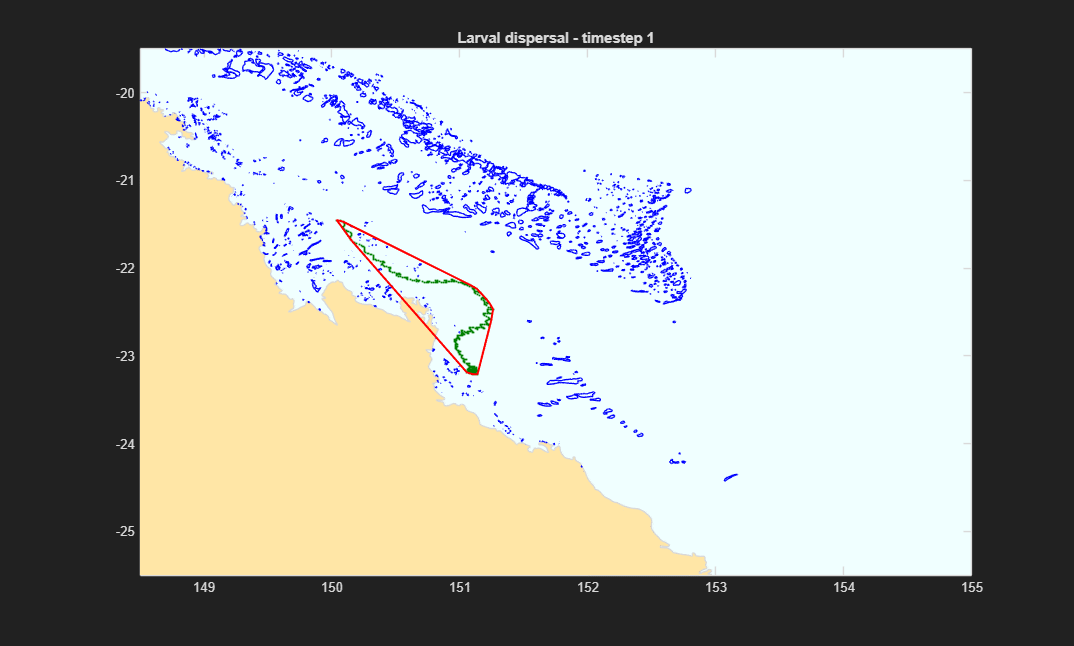
\includegraphics[width=0.48\linewidth,height=0.36\textheight,keepaspectratio]{figures/larvae_0.png}
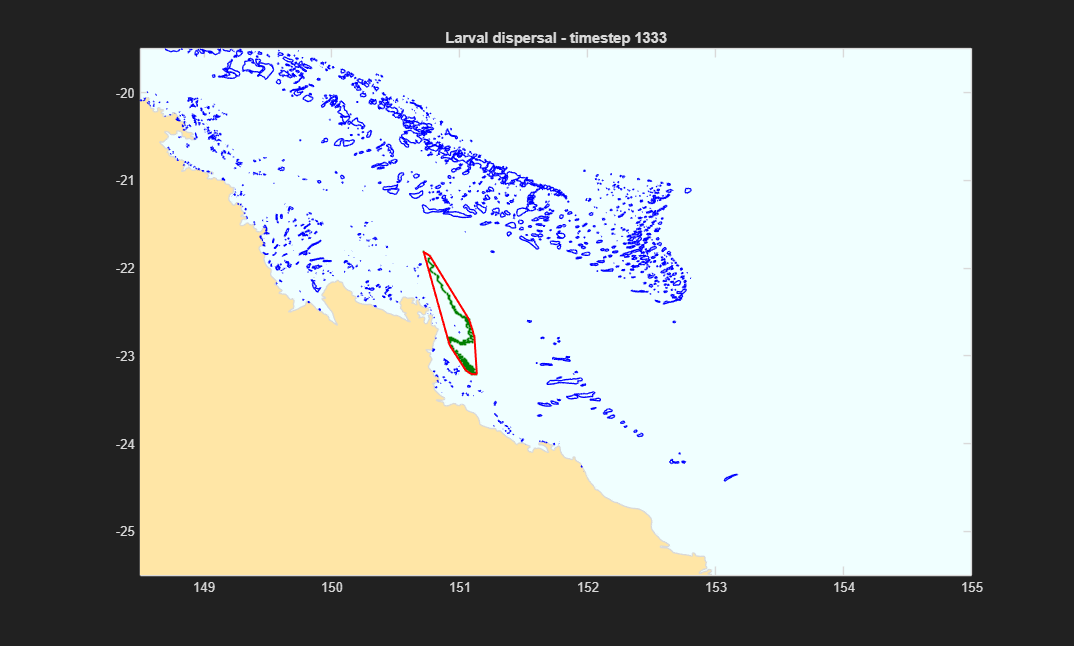
\includegraphics[width=0.48\linewidth,height=0.36\textheight,keepaspectratio]{figures/larvae_1.png}\par\vspace{4mm}
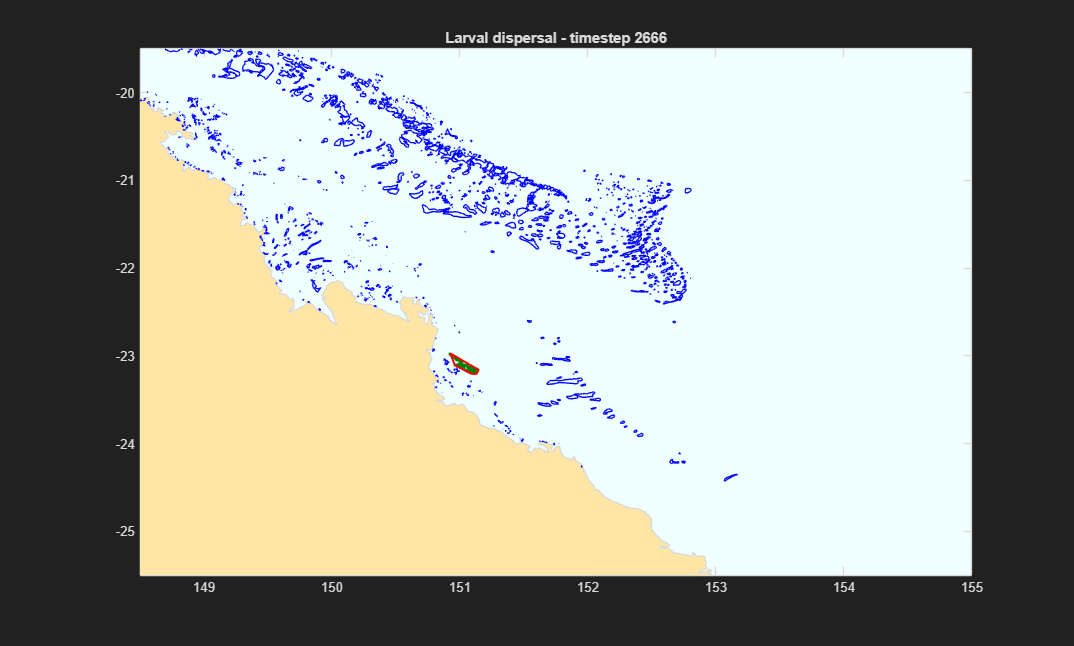
\includegraphics[width=0.48\linewidth,height=0.36\textheight,keepaspectratio]{figures/larvae_2.png}
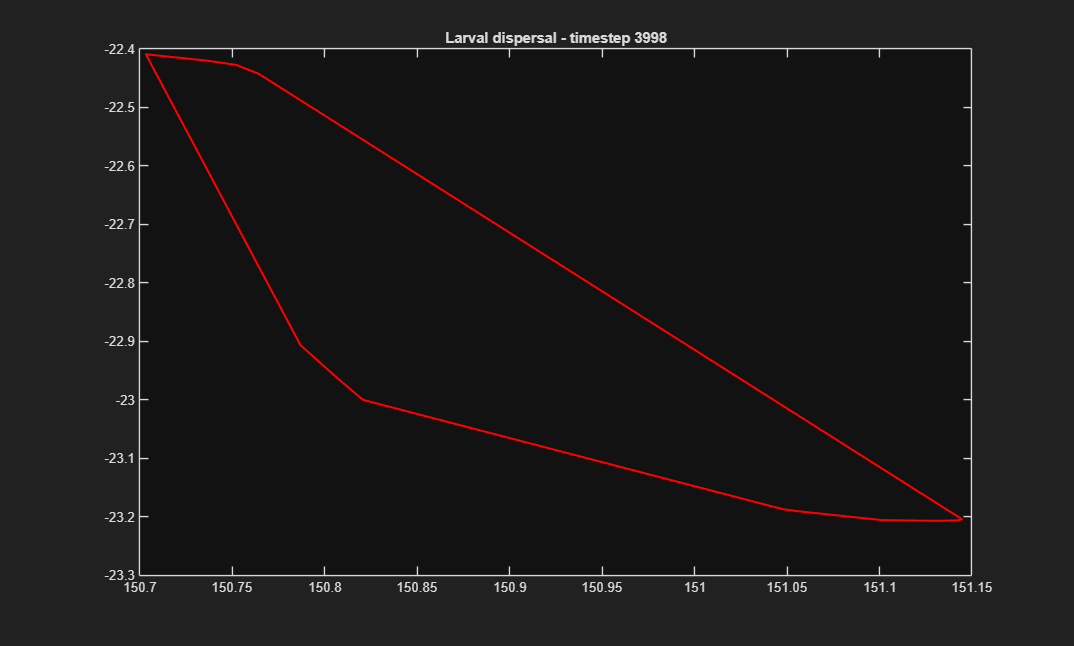
\includegraphics[width=0.48\linewidth,height=0.36\textheight,keepaspectratio]{figures/larvae_3.png}\par\vspace{4mm}
\end{center}Frames sampled at the beginning, approximately one-third and two-thirds through, and the end of the animation.
\task{Week 9 -- Fishery uncertainty}{Task 2: Show demographic, structural / parametric and scenario uncertainty in a labelled TIFF with legends.}
\needspace{35mm}{\large\bfseries\color{blue} Task 2 -- R fishery simulations}\par{\small Source: \texttt{week9/P9Task2.R}}\par
\lstinputlisting{../week9/P9Task2.R}
The stochastic simulation uses 2,500 replicates over 50 time steps; its shaded interval spans the 2.5th to 97.5th percentiles.
\figpage{Task 2 -- Three forms of uncertainty}{figures/fishery.png}{Original output: \texttt{week9/Fishery\_Uncertainty.tiff}. Structural uncertainty compares z = 1 and z = 2; scenario uncertainty compares h = 0.1 and h = 0.2. This PDF shows a lossless display conversion of the TIFF.}
\task{Week 10 -- Vector Visualisation}{Tasks 1--3: Direct vector field visualisation, poor and improved streamlines, and line integral convolution.}
\needspace{35mm}{\large\bfseries\color{blue} Tasks 1--3 -- Complete R code}\par{\small Source: \texttt{week10/week10\_vectors.R}}\par
\lstinputlisting{../week10/week10_vectors.R}
The complete R implementation includes the common interpolation, integration and export functions.
\figpage{Task 1 -- Direct vector field}{../week10/outputs/task1_quiver.pdf}{Quiver visualisation of the gradient of z = x exp(-x squared - y squared), sampled at grid spacing 0.1. Arrow orientation shows gradient direction and colour shows its magnitude.}
\figpage{Task 2 -- Poor streamline visualisation}{../week10/outputs/task2_poor_streamlines.pdf}{Nine regularly spaced seeds, 20 integration steps in each direction, step multiplier 0.5. Short paths and sparse seeds leave much of the flow structure unresolved.}
\figpage{Task 2 -- Improved streamline visualisation}{../week10/outputs/task2_good_streamlines.pdf}{361 regularly spaced seeds, 600 integration steps in each direction, step multiplier 0.5. Bilinear velocity interpolation and midpoint integration improve smoothness; integration stops at the domain boundary. Orange points mark seeds.}
\figpage{Task 3 -- Line integral convolution}{../week10/outputs/task3_lic.pdf}{Every grid point is a seed. Integration uses up to 30 steps each way at unit step size. Both optional extensions are implemented: normalised velocity and division by the actual sample count near boundaries. Display contrast is clipped at the 1st and 99th percentiles; the original LIC values are saved separately.}
\figpage{Task 3 -- Additional starting texture}{../week10/outputs/task3_noise.pdf}{Starting white noise generated with seed 362, before convolution along the vector field.}
\task{Week 11 -- Visualising High Dimensional Data}{Tasks 1--4: Iris scatter plot matrix, covariance-based PCA, and LDA projection and species separation.}

\needspace{35mm}{\large\bfseries\color{blue} Tasks 1--4 -- R code}\par{\small Source: \texttt{submission/code/week11\_corrected.R (run from week11)}}\par
\lstinputlisting[lastline=26]{code/week11_corrected.R}
The code produces the species-coloured iris scatter plot matrix and projects the mean-centred data onto the two principal components with the largest eigenvalues.

\clearpage{\Large\bfseries\color{navy} Week 11 -- LDA code}\par
\lstinputlisting[firstline=27,firstnumber=27]{code/week11_corrected.R}
The LDA examples in slides 6--7 use columns 1 and 3 (sepal length and petal length), while the final task slide asks for the first two dimensions. Both variable selections are supplied. The projection search evaluates unit vectors over 1,000 angles from 0 to pi, using between-class covariance divided by total covariance.
\figpage{Task 1 -- Iris scatter plot matrix}{figures/week11_pairs.png}{All six distinct pairs of the four numerical iris variables are displayed. Species are distinguished by both colour and symbol; duplicate lower-triangle panels are omitted.}
\figpage{Task 2 -- Principal component projection}{figures/week11_pca.png}{The mean-centred four-variable iris data are projected onto the two eigenvectors of the covariance matrix with the largest eigenvalues, with species indicated by colour and symbol.}
\task{Task 3 -- LDA projection results}{The reported vectors have unit length. J(W) is the Fisher criterion implemented in the code. Reversing both signs of W gives the same separation and criterion value.}
\begin{lstlisting}
Variables: Sepal.Length, Petal.Length
W = [-0.21989222; 0.97552417]
J(W) = 0.95251145

Variables: Sepal.Length, Sepal.Width
W = [-0.82674458; 0.56257746]
J(W) = 0.80126605

\end{lstlisting}
The first result follows the worked LDA instructions (columns 1 and 3). The second follows the final task wording literally (columns 1 and 2). Each corresponding species histogram follows.
\figpage{Task 4 -- LDA projection direction}{figures/week11_lda_direction_main.png}{Standardised sepal length and petal length, following slides 6--7. The black line gives the optimised projection direction.}
\figpage{Task 4 -- Species separation along W}{figures/week11_lda_histogram_main.png}{Histogram of projections onto the optimised vector for sepal length and petal length. Setosa separates clearly; versicolor and virginica overlap.}
\figpage{Tasks 3--4 -- First two dimensions}{figures/week11_lda_histogram_first_two.png}{Supplementary histogram for sepal length and sepal width, covering the final task slide wording. The matching W and J(W) are reported above.}
\end{document}